% f2015tjw_q17_solid.tex —— 2015 天津文科卷 Q17 立体图（源 p2 栏 1）
%
% 源：.work/phase3-b10/source/2015天津文.pdf（p2 印 988）；实测清单 figure-inventory.md §F04
% 坐标换算：x_pic = x_pt − 285.0 ；y_pic = 370.0 − y_pt
%   （源页 pt、原点左上、y 向下；画布 x' 2.7–120.2、y' 6.0–218.2，单位 pt）
% 线宽：0.3985 pt（源 `0.3985 w` 实测）；虚线用源 dash 实测节距 `[ 2.98883 2.98883 ] 0 d`
%   → dash pattern = on 2.98883pt off 2.98883pt（全卷仅本图 4 条棱为虚线）。
% 顶点（源 pt → 图内）：
%   B(299.659,320.463)→(14.659,49.537)  A(389.780,320.463)→(104.780,49.537)
%   C(367.328,351.335)→(82.328,18.665)  A₁(389.780,240.632)→(104.780,129.368)
%   B₁(299.659,160.802)→(14.659,209.198) E(333.493,335.899)→(48.493,34.101)
%   F(378.242,295.984)→(93.242,74.016)
% 实虚分工照源（不做修正）：7 实（BC、CA、B₁B、AA₁、CA₁、CB₁、A₁B₁）＋
%   4 虚（BA 底面棱、EA₁、EF、AE）＝ 11 条棱（源 22 条路径 = 11 棱 + 11 条退化 m 占位）。
% 存疑照源复刻：§S-6 F 点实测 (378.242,295.984) 与 A₁C 理论中点 (378.554,295.984) 差 x 0.312 pt；
%   E 点为 BC 中点（与题干一致，差 0.001 pt）——均按实测坐标给出。
% 全图无箭头（源 p2 图形线素无 f 填充箭尖）。
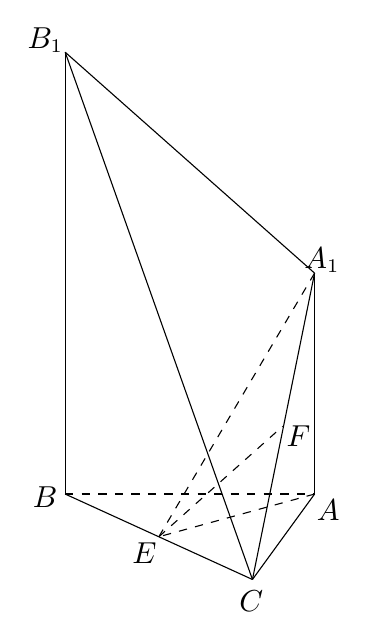
\begin{tikzpicture}[x=1pt, y=1pt, line width=0.3985pt, every node/.style={font=\fontsize{10.5pt}{12.6pt}\selectfont,inner sep=0pt}]

  % ---- 实线棱 7 条 ----
  \draw (14.659, 49.537) -- (82.328, 18.665);   % E1  B -> C
  \draw (82.328, 18.665) -- (104.780,49.537);   % E2  C -> A
  \draw (14.659,209.198) -- (14.659, 49.537);   % E3  B1 -> B
  \draw (104.780,49.537) -- (104.780,129.368);  % E4  A -> A1
  \draw (82.328, 18.665) -- (104.780,129.368);  % E5  C -> A1
  \draw (82.328, 18.665) -- (14.659,209.198);   % E6  C -> B1
  \draw (104.780,129.368) -- (14.659,209.198);  % E7  A1 -> B1

  % ---- 虚线棱 4 条（dash 2.98883 on/off，源实测） ----
  \draw[dash pattern=on 2.98883pt off 2.98883pt] (14.659,49.537) -- (104.780,49.537);   % E8  B -> A（底面）
  \draw[dash pattern=on 2.98883pt off 2.98883pt] (48.493,34.101) -- (104.780,129.368);  % E9  E -> A1
  \draw[dash pattern=on 2.98883pt off 2.98883pt] (48.493,34.101) -- (93.242, 74.016);   % E10 E -> F
  \draw[dash pattern=on 2.98883pt off 2.98883pt] (104.780,49.537) -- (48.493,34.101);   % E11 A -> E

  % ---- 标签（源标签 bbox 中心 → 最近顶点判定归属；anchor=center、inner sep=0） ----
  \node[anchor=center,inner sep=0] at (  7.42,48.57) {$B$};
  \node[anchor=center,inner sep=0] at (109.71,43.64) {$A$};
  \node[anchor=center,inner sep=0] at ( 81.95,10.73) {$C$};
  \node[anchor=center,inner sep=0] at (107.48,134.12) {$A_1$};
  \node[anchor=center,inner sep=0] at (  7.50,213.50) {$B_1$};
  \node[anchor=center,inner sep=0] at ( 43.26,28.21) {$E$};
  \node[anchor=center,inner sep=0] at ( 98.96,70.38) {$F$};

\end{tikzpicture}
